\chapter{Testing Environment \& Results} \label{ap2:testing}

\section{webMUSHRA Testing}

\begin{figure}[H]
    \centering
    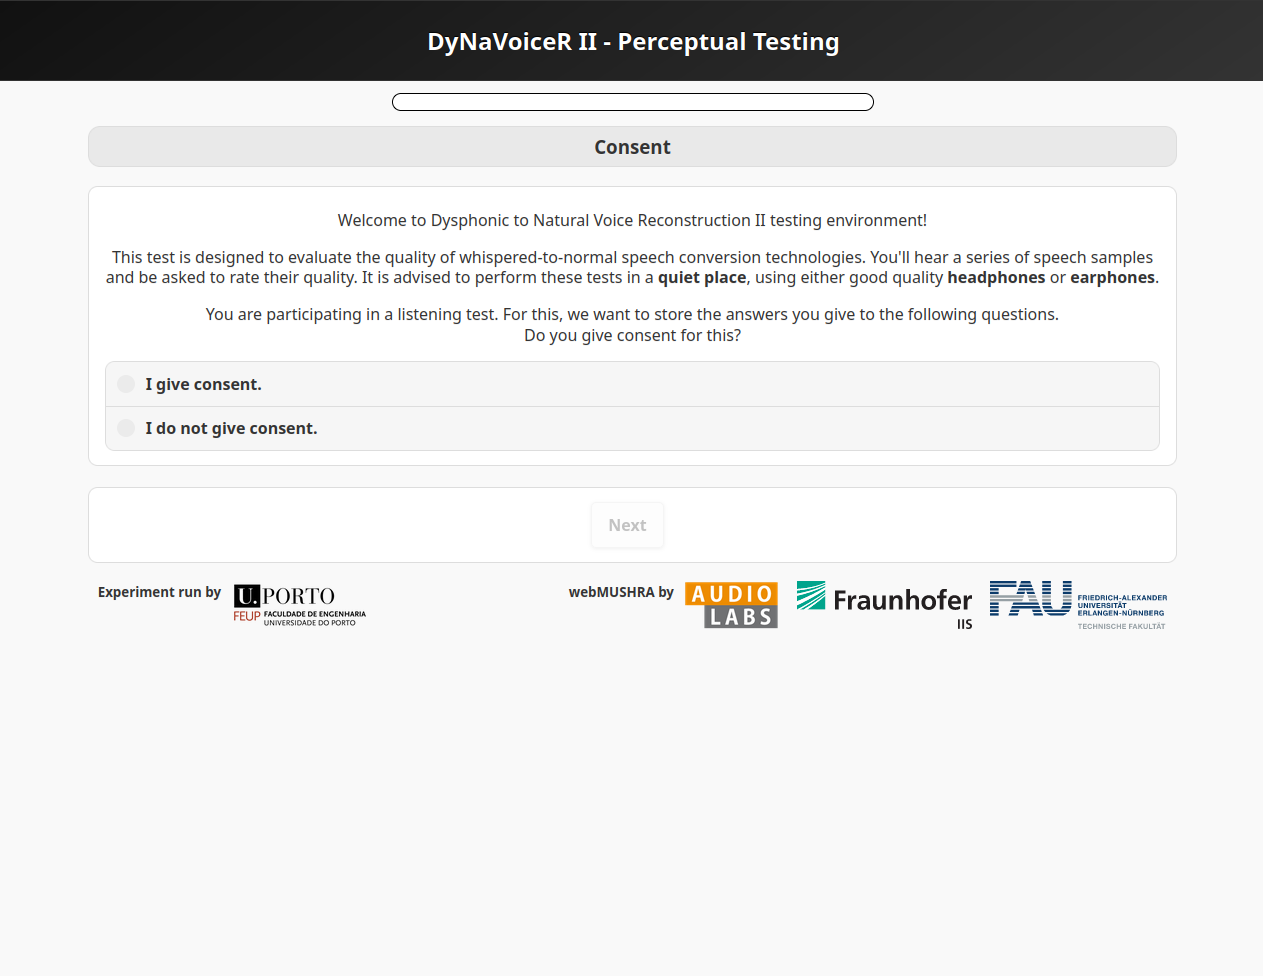
\includegraphics[width=\textwidth]{chapter7/consent.png}
    \caption{Test introduction, contextualization and consent form}
    \label{fig:consent}
\end{figure}

\begin{figure}[H]
    \centering
    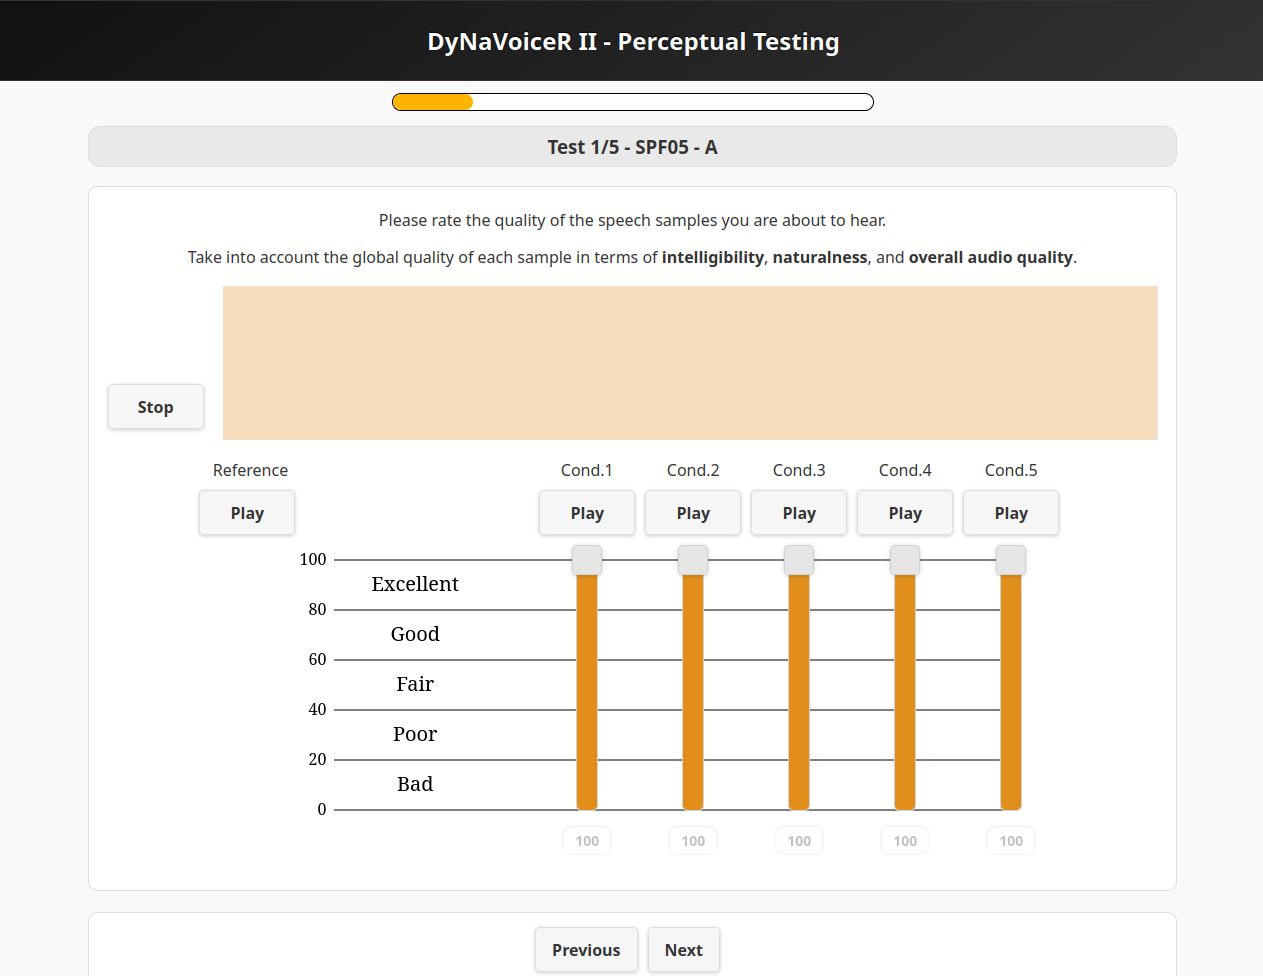
\includegraphics[width=\textwidth]{chapter7/w2s.png}
    \caption{Whispered to Speech test page}
    \label{fig:mushraW2C}
\end{figure}

\begin{figure}[H]
    \centering
    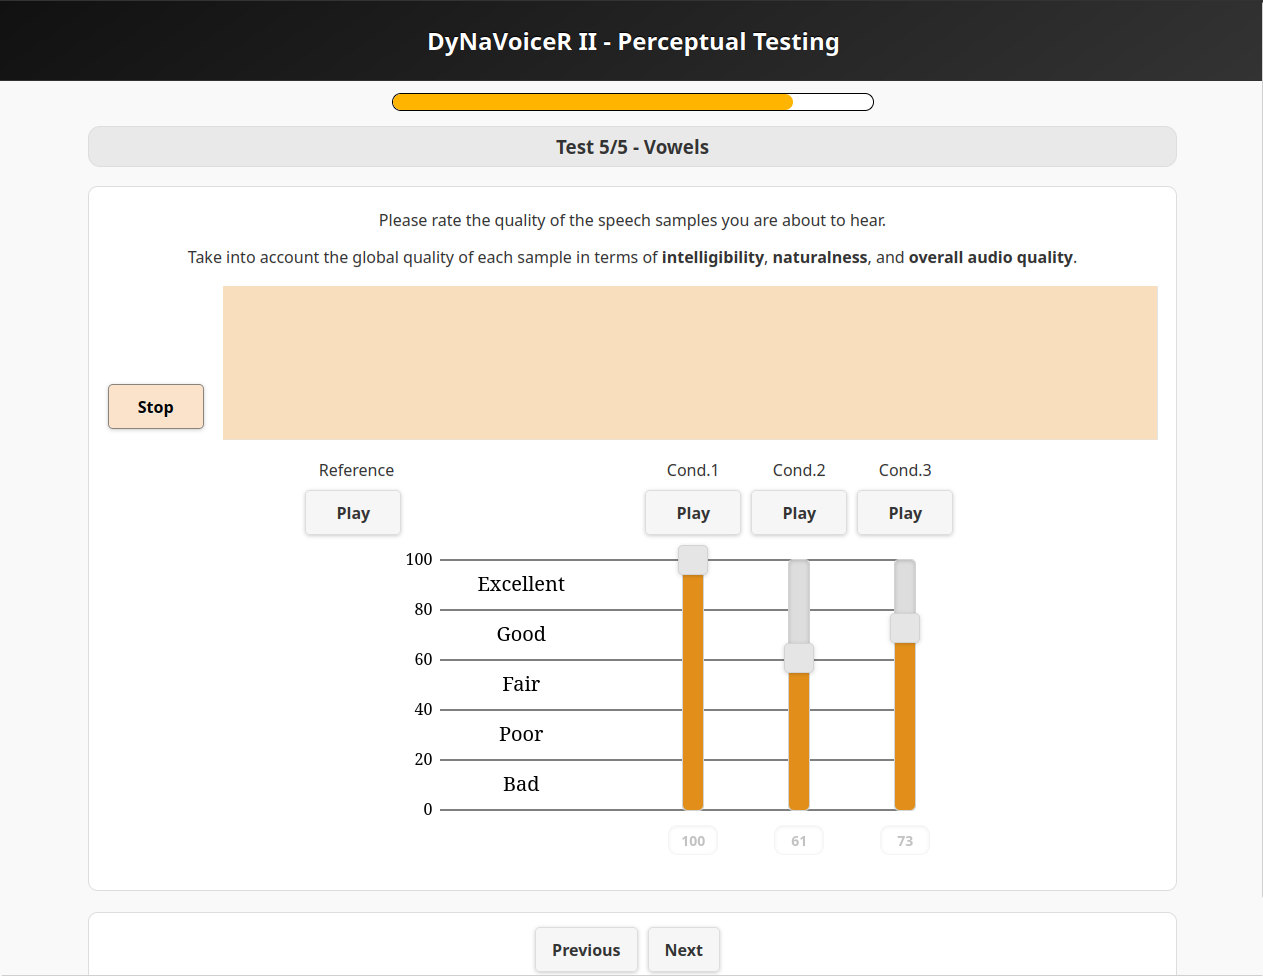
\includegraphics[width=\textwidth]{chapter7/vowel.png}
    \caption{Synthetic vowel test page}
    \label{fig:mushraVowel}
\end{figure}

\begin{figure}[H]
    \centering
    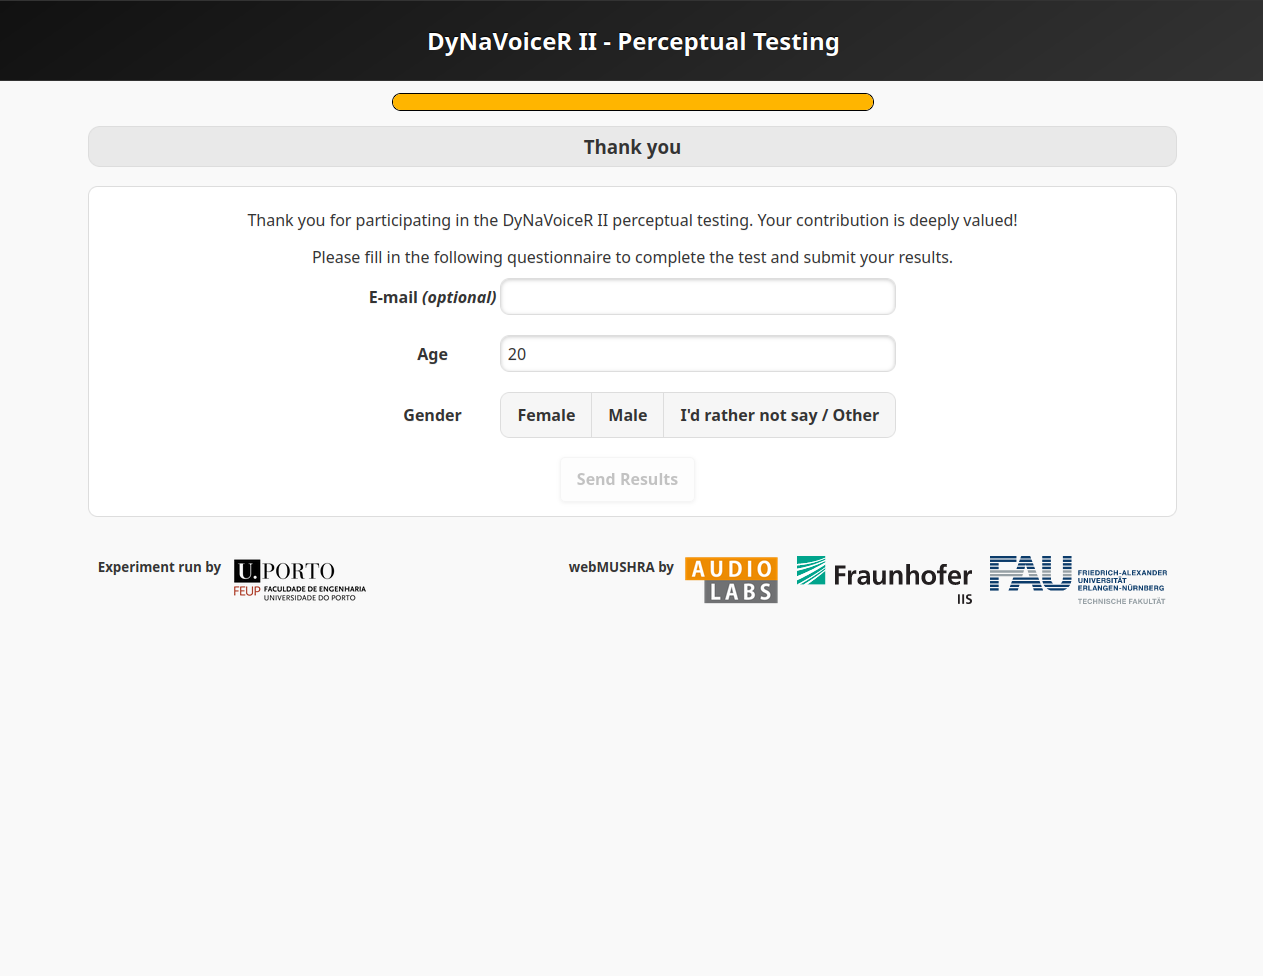
\includegraphics[width=\textwidth]{chapter7/final.png}
    \caption{Final page with feedback form}
    \label{fig:final}
\end{figure}

\section{t-Testing results}

\begin{table}[H]
    \centering
    \begin{tabular}{lccccc}
        \hline
        & Reference & Whispered & FrameFilt & PulseFilt & Segmented \\
        \hline
        Reference & - & 4.46e-02 & 1.77e-12 & 6.83e-13 & 1.34e-09 \\
        Whispered & 4.46e-02 & - & 3.94e-11 & 5.23e-09 & 2.45e-07 \\
        FrameFilt & 1.77e-12 & 3.94e-11 & - & 2.07e-01 & 9.81e-07 \\
        PulseFilt & 6.83e-13 & 5.23e-09 & 2.07e-01 & - & 5.22e-06 \\
        Segmented & 1.34e-09 & 2.45e-07 & 9.81e-07 & 5.22e-06 & - \\
        \hline
    \end{tabular}
    \caption{Pairwise P-Values for subject SPF05}
    \label{tab:pairwiseSPF05}
\end{table}

\begin{table}[H]
    \centering
    \begin{tabular}{lccccc}
        \hline
        & Reference & Whispered & FrameFilt & PulseFilt & Segmented \\
        \hline
        Reference & - & 7.04e-03 & 5.12e-13 & 3.68e-13 & 7.62e-10 \\
        Whispered & 7.04e-03 & - & 1.88e-11 & 1.68e-08 & 2.00e-06 \\
        FrameFilt & 5.12e-13 & 1.88e-11 & - & 1.00e-01 & 4.45e-04 \\
        PulseFilt & 3.68e-13 & 1.68e-08 & 1.00e-01 & - & 1.41e-03 \\
        Segmented & 7.62e-10 & 2.00e-06 & 4.45e-04 & 1.41e-03 & - \\
        \hline
    \end{tabular}
    \caption{Pairwise P-Values for subject SPF12}
    \label{tab:pairwiseSPF12}
\end{table}

\begin{table}[H]
    \centering
    \begin{tabular}{lccccc}
        \hline
        & Reference & Whispered & FrameFilt & PulseFilt & Segmented \\
        \hline
        Reference & - & 1.34e-02 & 2.70e-12 & 5.35e-12 & 1.82e-09 \\
        Whispered & 1.34e-02 & - & 1.05e-09 & 9.62e-09 & 4.17e-07 \\
        FrameFilt & 2.70e-12 & 1.05e-09 & - & 1.49e-01 & 7.39e-05 \\
        PulseFilt & 5.35e-12 & 9.62e-09 & 1.49e-01 & - & 3.95e-04 \\
        Segmented & 1.82e-09 & 4.17e-07 & 7.39e-05 & 3.95e-04 & - \\
        \hline
    \end{tabular}
    \caption{Pairwise P-Values for subject SPM14}
    \label{tab:pairwiseSPM14}
\end{table}

\begin{table}[H]
    \centering
    \begin{tabular}{lccccc}
        \hline
        & Reference & Whispered & FrameFilt & PulseFilt & Segmented \\
        \hline
        Reference & - & 5.70e-02 & 4.95e-11 & 4.71e-11 & 2.55e-08 \\
        Whispered & 5.70e-02 & - & 6.99e-11 & 1.06e-09 & 1.03e-06 \\
        FrameFilt & 4.95e-11 & 6.99e-11 & - & 5.82e-01 & 8.17e-04 \\
        PulseFilt & 4.71e-11 & 1.06e-09 & 5.82e-01 & - & 5.95e-05 \\
        Segmented & 2.55e-08 & 1.03e-06 & 8.17e-04 & 5.95e-05 & - \\
        \hline
    \end{tabular}
    \caption{Pairwise P-Values for subject SPM18}
    \label{tab:pairwiseSPM18}
\end{table}